\documentclass[border=8pt]{standalone}
\usepackage{tikz}
\usepackage{amsmath}
\usetikzlibrary{arrows.meta, positioning, calc}

\definecolor{cBlur}{RGB}{129,145,222}
\definecolor{cAccentSigma}{RGB}{201,150,20}   % Kupfer/Gold -- Sigma
\definecolor{cAccentRadius}{RGB}{58,140,99}   % Gruen -- Radius
\definecolor{boxbg}{RGB}{250,250,248}

\begin{document}
    \begin{tikzpicture}[
        scale=0.75,
        every node/.style={transform shape},
        pixel/.style={rectangle, draw, minimum size=1.3cm, align=center, font=\small, inner sep=2pt},
        k_low/.style={pixel,  fill=cBlur!25},
        k_mid/.style={pixel,  fill=cBlur!45},
        k_high/.style={pixel, fill=cBlur!70},
        callout/.style={rectangle, rounded corners=2pt, draw, line width=1.4pt,
        fill=boxbg, align=left, font=\scriptsize, inner sep=7pt, text width=9cm,
        anchor=north},
        tag/.style={font=\scriptsize\bfseries},
        swatch/.style={rectangle, draw, minimum size=4.5mm, inner sep=0pt}
    ]

        \node[k_low]  at (0,0)      {0.0894};
        \node[k_mid]  at (1.4,0)    {0.1201};
        \node[k_low]  at (2.8,0)    {0.0894};
        \node[k_mid]  at (0,-1.4)   {0.1201};
        \node[k_high] at (1.4,-1.4) {0.1615};
        \node[k_mid]  at (2.8,-1.4) {0.1201};
        \node[k_low]  at (0,-2.8)   {0.0894};
        \node[k_mid]  at (1.4,-2.8) {0.1201};
        \node[k_low]  at (2.8,-2.8) {0.0894};

        \draw[cAccentSigma, line width=1.2pt, dashed, rounded corners=3pt]
        (-0.75,0.75) rectangle (3.55,-3.55);
        \node[tag, text=cAccentSigma] at (1.4,1.1) {Gaussian-Kernel (Gewichte)};

        \node[font=\Large] at (6.95,-1.4) {$\times$};

        \node[pixel, fill=black!90, text=white] at (11.1,0)    {L10};
        \node[pixel, fill=black!70, text=white] at (12.5,0)    {L20};
        \node[pixel, fill=black!50, text=white] at (13.9,0)    {L30};
        \node[pixel, fill=black!45, text=white] at (11.1,-1.4) {L50};
        \node[pixel, fill=black!50, text=white] at (12.5,-1.4) {L48};
        \node[pixel, fill=black!90, text=white] at (13.9,-1.4) {L10};
        \node[pixel, fill=black!10]             at (11.1,-2.8) {L90};
        \node[pixel, fill=black!60, text=white] at (12.5,-2.8) {L30};
        \node[pixel, fill=black!70, text=white] at (13.9,-2.8) {L20};

        \draw[cAccentRadius, line width=1.2pt, dashed, rounded corners=3pt]
        (10.35,0.75) rectangle (14.65,-3.55);
        \node[tag, text=cAccentRadius] at (12.5,1.1) {Bildausschnitt (Nachbarschaft)};

        \node[font=\Large] at (17.75,-1.4) {$=$};

        \node[pixel, fill=black!52, text=white] at (21.5,-1.4) {L34};

        \node[callout, draw=cAccentSigma] (sigmabox) at (1.4,-4.0)
            {
            \textbf{\textcolor{cAccentSigma}{$\sigma$ :}} bestimmt die \emph{Form} der Gewichtsverteilung im Kernel.

            \vspace{4pt}
            \begin{center}
                \fbox{\resizebox{2.6cm}{!}{$\displaystyle G(x) = \exp\!\left(-\frac{x^2}{2\sigma^2}\right)$}}
            \end{center}
            \vspace{4pt}

            Kleines $\sigma$ $\rightarrow$ Gewicht stark auf das Zentrum konzentriert.

            \vspace{3pt}
            \begin{tikzpicture}[baseline, every node/.style={font=\tiny}]
            \node[anchor=west] at (0,0) {          };
            \foreach \i/\c in {0/15, 1/55, 2/95, 3/55, 4/15}{
                \node[swatch, fill=cAccentSigma!\c] at (1.55+0.42*\i,0) {};
            }
            \end{tikzpicture}

            \vspace{4pt}
            Gro{\ss}es $\sigma$ $\rightarrow$ Gewichte flacher verteilt.

            \vspace{3pt}
            \begin{tikzpicture}[baseline, every node/.style={font=\tiny}]
            \node[anchor=west] at (0,0) {          };
            \foreach \i/\c in {0/45, 1/55, 2/65, 3/55, 4/45}{
                \node[swatch, fill=cAccentSigma!\c] at (1.55+0.42*\i,0) {};
            }
            \end{tikzpicture}
        };

        \node[callout, draw=cAccentRadius] (radiusbox) at (12.5,-4.0)
            {
            \textbf{\textcolor{cAccentRadius}{\texttt{blur\_radius}:}} bestimmt die \emph{Gr{\"o}{\ss}e} des Kernels bzw. der betrachteten Nachbarschaft.

            \vspace{4pt}
            \begin{center}
                \fbox{\resizebox{3.4cm}{!}{$\displaystyle \text{Kernelbreite} = 2\cdot\texttt{blur\_radius}+1$}}
            \end{center}
            \vspace{4pt}

            \texttt{blur\_radius = 1} $\rightarrow$ $3\times3$-Kernel (8 Nachbarn).

            \vspace{2pt}
            Gr{\"o}{\ss}erer Radius $\rightarrow$ mehr Nachbarpixel, mehr Rechenaufwand.

            \vspace{5pt}
            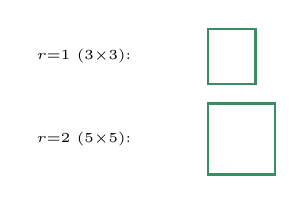
\begin{tikzpicture}[baseline, every node/.style={font=\tiny}]
            \node[anchor=west] at (0,0.45) {$r{=}1$ ($3{\times}3$):};
            \draw[cAccentRadius, line width=0.9pt] (2.3,0.1) rectangle (2.9,0.8);

            \node[anchor=west] at (0,-0.6) {$r{=}2$ ($5{\times}5$):};
            \draw[cAccentRadius, line width=0.9pt] (2.3,-1.05) rectangle (3.15,-0.15);
            \end{tikzpicture}
        };

    \end{tikzpicture}
\end{document}